\chapter{Koncepce hry}
\label{chap:analysis}
Návrh implementované hry zakládá na analýze hry Berušky 2, která byla provedena metodou \textit{černé skříňky}\footnote{Na základě akcí uživatele byla zkoumána reakce hry s tím, že princip vnitřní implementace zůstal utajen.}. Hra je nejprve stručně představena a následně jsou uvedeny výsledky herní analýzy, na kterých zakládá implementace~\ref{chap:implementace}

\section{Berušky 2}
Berušky 2, neboli také Berušky 3D, jsou pokračováním logické hry vývojářského týmu Anakreon\footnote{\url{www.anakreon.cz}}, jehož členem je pan Ing. Martin Stránský, který byl konzultantem této bakalářské práce. Oproti své první, volně dostupné verzi, bylo toto pokračování od počátku vytvářeno jako komerční produkt. Hra byla od roku 2004 distribuována v České republice a některých dalších zemích společností Cinemax. V březnu roku 2011 byla část této hry uvolněna pod open-source licencí a je dále vyvíjena panem Stránským. První verze hry Berušky je svou koncepcí velmi podobná hře Sokoban~\footnote{\url{https://en.wikipedia.org/wiki/Sokoban}}. Druhá verze hry se svou koncepcí příliš od prvního dílu neodlišuje, avšak do hry přibyly nové herní prvky, a co je hlavní, hra je kompletně ve 3D. Každá úroveň této hry je logickou hříčkou, která ke svému řešení vyžaduje volbu správného plánu a dávku trpělivosti. Každá z berušek má schopnost před sebou tlačit bedny a používat herní předměty, čímž vytváří cestu k cíli, avšak pro jeho dosažení je často důležité, aby spolu berušky vzájemně spolupracovali.

Původní hra distribuovaná firmou Cinemax obsahuje celkově 160 herních úrovní včetně 20 tutoriálů a 45 jednodušších úrovní, které jsou určeny pro mladší hráče a trénink. Hlavní součástí hry je pak \textit{Beruščí cesta}, která obsahuje celkem 95 úrovní rozdělených do 9 epizod odehrávajících se v různých prostředích. Open-source verze hry pak obsahuje tutoriály, některé tréninkové úrovně a 3 z úrovní Beruščí cesty.

\section{Herní pole}
Herní pole je ve tvaru krychle či kvádru a je rozděleno na jednotlivé pozice, ve kterých jsou umístěny jeho prvky (diagram~\ref{fig:gameField}). Nikdy nemůže dojít k situaci, že by se herní prvek včetně berušek vyskytl mimo herní pole. Po prvcích jako jsou bedny, či zeď je možné se volně pohybovat, avšak beruška nikdy nemůže z vyšší herní pozice seskočit dolů.

\begin{figure}[htb]
\centering
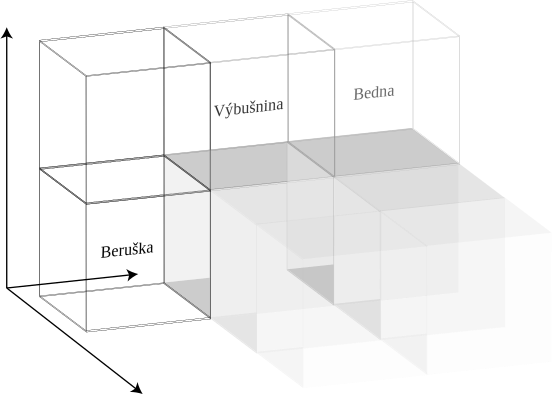
\includegraphics[width=0.8\textwidth]{gameField}
\caption{Herní pole a jeho prvky}
\label{fig:gameField}
\end{figure}

\section{Prvky herního pole}
Jak již bylo uvedeno, v rámci herního pole jsou umístěny prvky, jejichž rozmístění představuje samotnou logickou hříčku, kterou hráč řeší. Prvky se od sebe liší nejen funkčností a vzhledem, ale také tím, že některé z nich jsou umístěny staticky (hráč s nimi nemůže pohnout) a některé z nich jsou dynamické (bedny, výbušniny, \ldots). Následuje přehled prvků herního pole a jejich stručný popis.

\myparagraph{Beruška}  %\item[Beruška] \hfill \\
V každé herní úrovni se vyskytuje 1-5 berušek, které jsou ovládány hráčem. Berušky mohou pohybovat bednami, či výbušninami za účelem vytvoření cesty k východu. Každá z nich má inventář, který obsahuje předměty, které beruška při svém pohybu herním polem získala. 
\myparagraph{Zeď}  %\item[Zeď] \hfill \\
Zeď je jedním ze statických prvků, který má ve svém herním poli stálou pozici a nelze ho nijak odstranit. Beruška se po zdech může volně pohybovat.
\myparagraph{Východ}  %\item[Východ] \hfill \\
Cílem je dostat všechny berušky do východu. Stejně jako zeď je i východ umístěn stále na stejné pozici.
\myparagraph{Bedna} % \item[Bedna] \hfill \\
Bedna je základním herním prvkem, který beruška tlačí před sebou a vytváří tak cestu k cíli. Počet přesouvaných beden je závislý na aktuální síle berušky (podkapitola~\ref{section:weight}) a je možné je odstranit pomocí výbušniny. Bedny lze také tlačit po šikmé podlaze a dostat je tak do vyšší, či nižší úrovně herního pole. Podle váhy pak rozlišujeme bedny na lehké a těžké.
\myparagraph{Výbušnina}%\item[Výbušnina] \hfill \\
Výbušnina je prvkem, který se po většinu času chová jako obyčejná bedna, avšak pokud je \uv{natlačena} na některou z beden, pak dojde k výbuchu. Bližší popis toho, jak výbuchy probíhají, je v podkapitole~\ref{section:explosive}.
\myparagraph{Kámen}%\item[Kámen] \hfill \\
Kámen představuje překážku, kterou nelze posunout, avšak je možné ho odstranit pomocí krompáče, který může beruška nalézt při průchodu herním polem.
\myparagraph{Voda}%\item[Voda] \hfill \\
Voda je pro berušku další překážkou. Pokud je v dané herní úrovni voda, pak musí beruška s největší pravděpodobností pod vodní hladinu, kde získá potřebný předmět. Někdy se dokonce pod vodní hladinou nachází i východ z úrovně, avšak v každém případě beruška potřebuje šnorchl, aby se mohla potopit. Ten může stejně jako krompáč získat při průchodu herním polem. 
\myparagraph{Krompáč}%\item[Krompáč] \hfill \\
Krompáč je předmět, který se používá pro odstranění kamene. Maximální počet krompáčů, který může mít jedna beruška v inventáři, je 4. Po použití je krompáč odstraněn z inventáře.
\myparagraph{Šnorchl}%\item[Šnorchl] \hfill \\
Beruška ho potřebuje, aby se mohla potopit pod vodní hladinu. Pokud beruška tento předmět nemá ve svém inventáři, pak je zamezeno jakémukoliv hernímu kroku, kterým by se beruška mohla pod hladinu dostat.
\myparagraph{Závaží}%\item[Závaží] \hfill \\
Závaží dvojnásobně zvyšuje váhu berušky. Toho se využívá v situacích, kdy potřebujeme, aby se pod beruškou propadla podlaha. 
\myparagraph{Hormonální vitamín}%\item[Hormonální vitamín] \hfill \\
Pokud beruška získá hormonální vitamín, pak získá dvojnásobnou sílu, což ji následně umožňuje před sebou tlačit více beden.
\myparagraph{Bortící se podlaha}%\item[Bortící se podlaha] \hfill \\
Občas se hře vyskytuje i podlaha, která se propadá pod vahou, která je nad ní naskladněna. Bližší informace o vahách herních prvků jsou uvedeny v podkapitole~\ref{section:weight}.
\myparagraph{Šikmina}%\item[Šikmina] \hfill \\
Šikmina je posledním z herních prvků. Umožňuje berušce sestoupit, či vystoupit z/do vyšší úrovně herního pole. Zároveň je možné po šikmině pohybovat bednami a výbušninami.

\section{Váhy herních prvků a síla berušky}
\label{section:weight}
Ve hře hraje velkou roli váha, která je přiřazena každému z prvků. Ta rozhoduje o tom, zda je beruška schopná posunout prvky, které se před ní nacházejí, a také o tom, zda se pod nimi nepropadne podlaha. Základní síla berušky, resp. to, kolik váhy před sebou může tlačit, jsou 2 váhové jednotky. S hormonálním vitamínem ve svém inventáři je pak síla berušky navýšena na 4 váhové jednotky. Bortící se podlaha nad sebou udrží pouze 1 váhovou jednotku a může na ni tedy být natlačena lehká bedna, nebo si na ni může stoupnout beruška, která ve svém inventáři nemá závaží. Při překročení váhy se podlaha propadne a objekty, které na ní byly naskládány, změní svou vertikální pozici tak, aby pod sebou měly podklad. Zajímají nás pouze váhy prvků, se kterými je možné ve hře pohybovat. Přehled dynamických prvků a jejich vah je uveden v tabulce~\ref{table:weights}.

\begin{table}
\label{table:weights}
\begin{center}
    \begin{tabular}{ | l | l |}
    \hline
    \textbf{Prvek} & \textbf{Váha} \\ \hline
    Beruška & 1 \\ \hline
    Lehká bedna & 1 \\ \hline
    Těžká bedna & 2 \\ \hline
	Výbušná bedna & 2 \\ \hline
    \end{tabular}

\end{center}
\caption{Váhy dynamických prvků}
\end{table}

\section{Posuvy beden}
Bedny jsou ve hře na různých pozicích a často jsou umístěny za sebou. O tom, zda beruška může provést posuv jedné či více beden rozhoduje více faktorů. 

\begin{itemize}
\item Aktuální beruščina síla. 
\item Obsah pozice za poslední posouvanou bednou.
\item Součet vah posouvaných beden.
\end{itemize} 

Pokud uvažujeme posuv jedné jediné bedny, pak je situace jednoduchá. Zjistí se obsah pozice, kam má být bedna posunuta, a pokud je tato pozice prázdná, pak se posun provede. Při posuvu více beden najednou je potřeba spočítat souhrnnou váhu posouvaných beden a určit obsah pozice, na kterou bude posunuta od berušky nejvzdálenější z nich. Jakmile má beruška dostatečnou sílu k posunu a konečná pozice je prázdná, pak je posun proveden. V opačném případě zůstává beruška i bedny na svém původním místě.

Je také důležité zdůraznit, že bedny mohou být posunuty do míst, kde pod sebou nemají žádný podklad. V takových situacích je pozice těchto beden upravena tak, aby pod sebou měly nějaký prvek.

\section{Výbušné bedny}
\label{section:explosive}
Výbušnými bednami lze ve většině situací normálně pohybovat. Změna nastává v případě, kdy je před výbušninou bedna obyčejná. V takové situaci je na ni výbušná bedna \uv{nasunuta} a dochází k výbuchu. Při výbuchu jsou obě bedny odstraněny a je upravena vertikální pozice prvků, které se nad nimi před výbuchem nacházely. Posouvanými prvky mohou být další výbušné bedny a ty při posunu vždy odstraní obyčejné, které se nacházejí pod nimi. 

Na diagramu~\ref{fig:bangDiagram} je ukázka komplexního výbuchu. Váha beden zde značně přesahuje beruščinu sílu, avšak za výbušnou bednou do které beruška tlačí je bedna obyčejná. Dojde tedy k výbuchu, odstranění beden a \uv{pádu} těch, které se nad nimi nacházely. Při pádu jsou odstraňovány bedny, které nad sebou mají výbušninu a zbude pouze jediná. Ta se nakonec bude nacházet přímo před beruškou, která zůstává na své původní pozici.

\begin{figure}[htb]
\centering
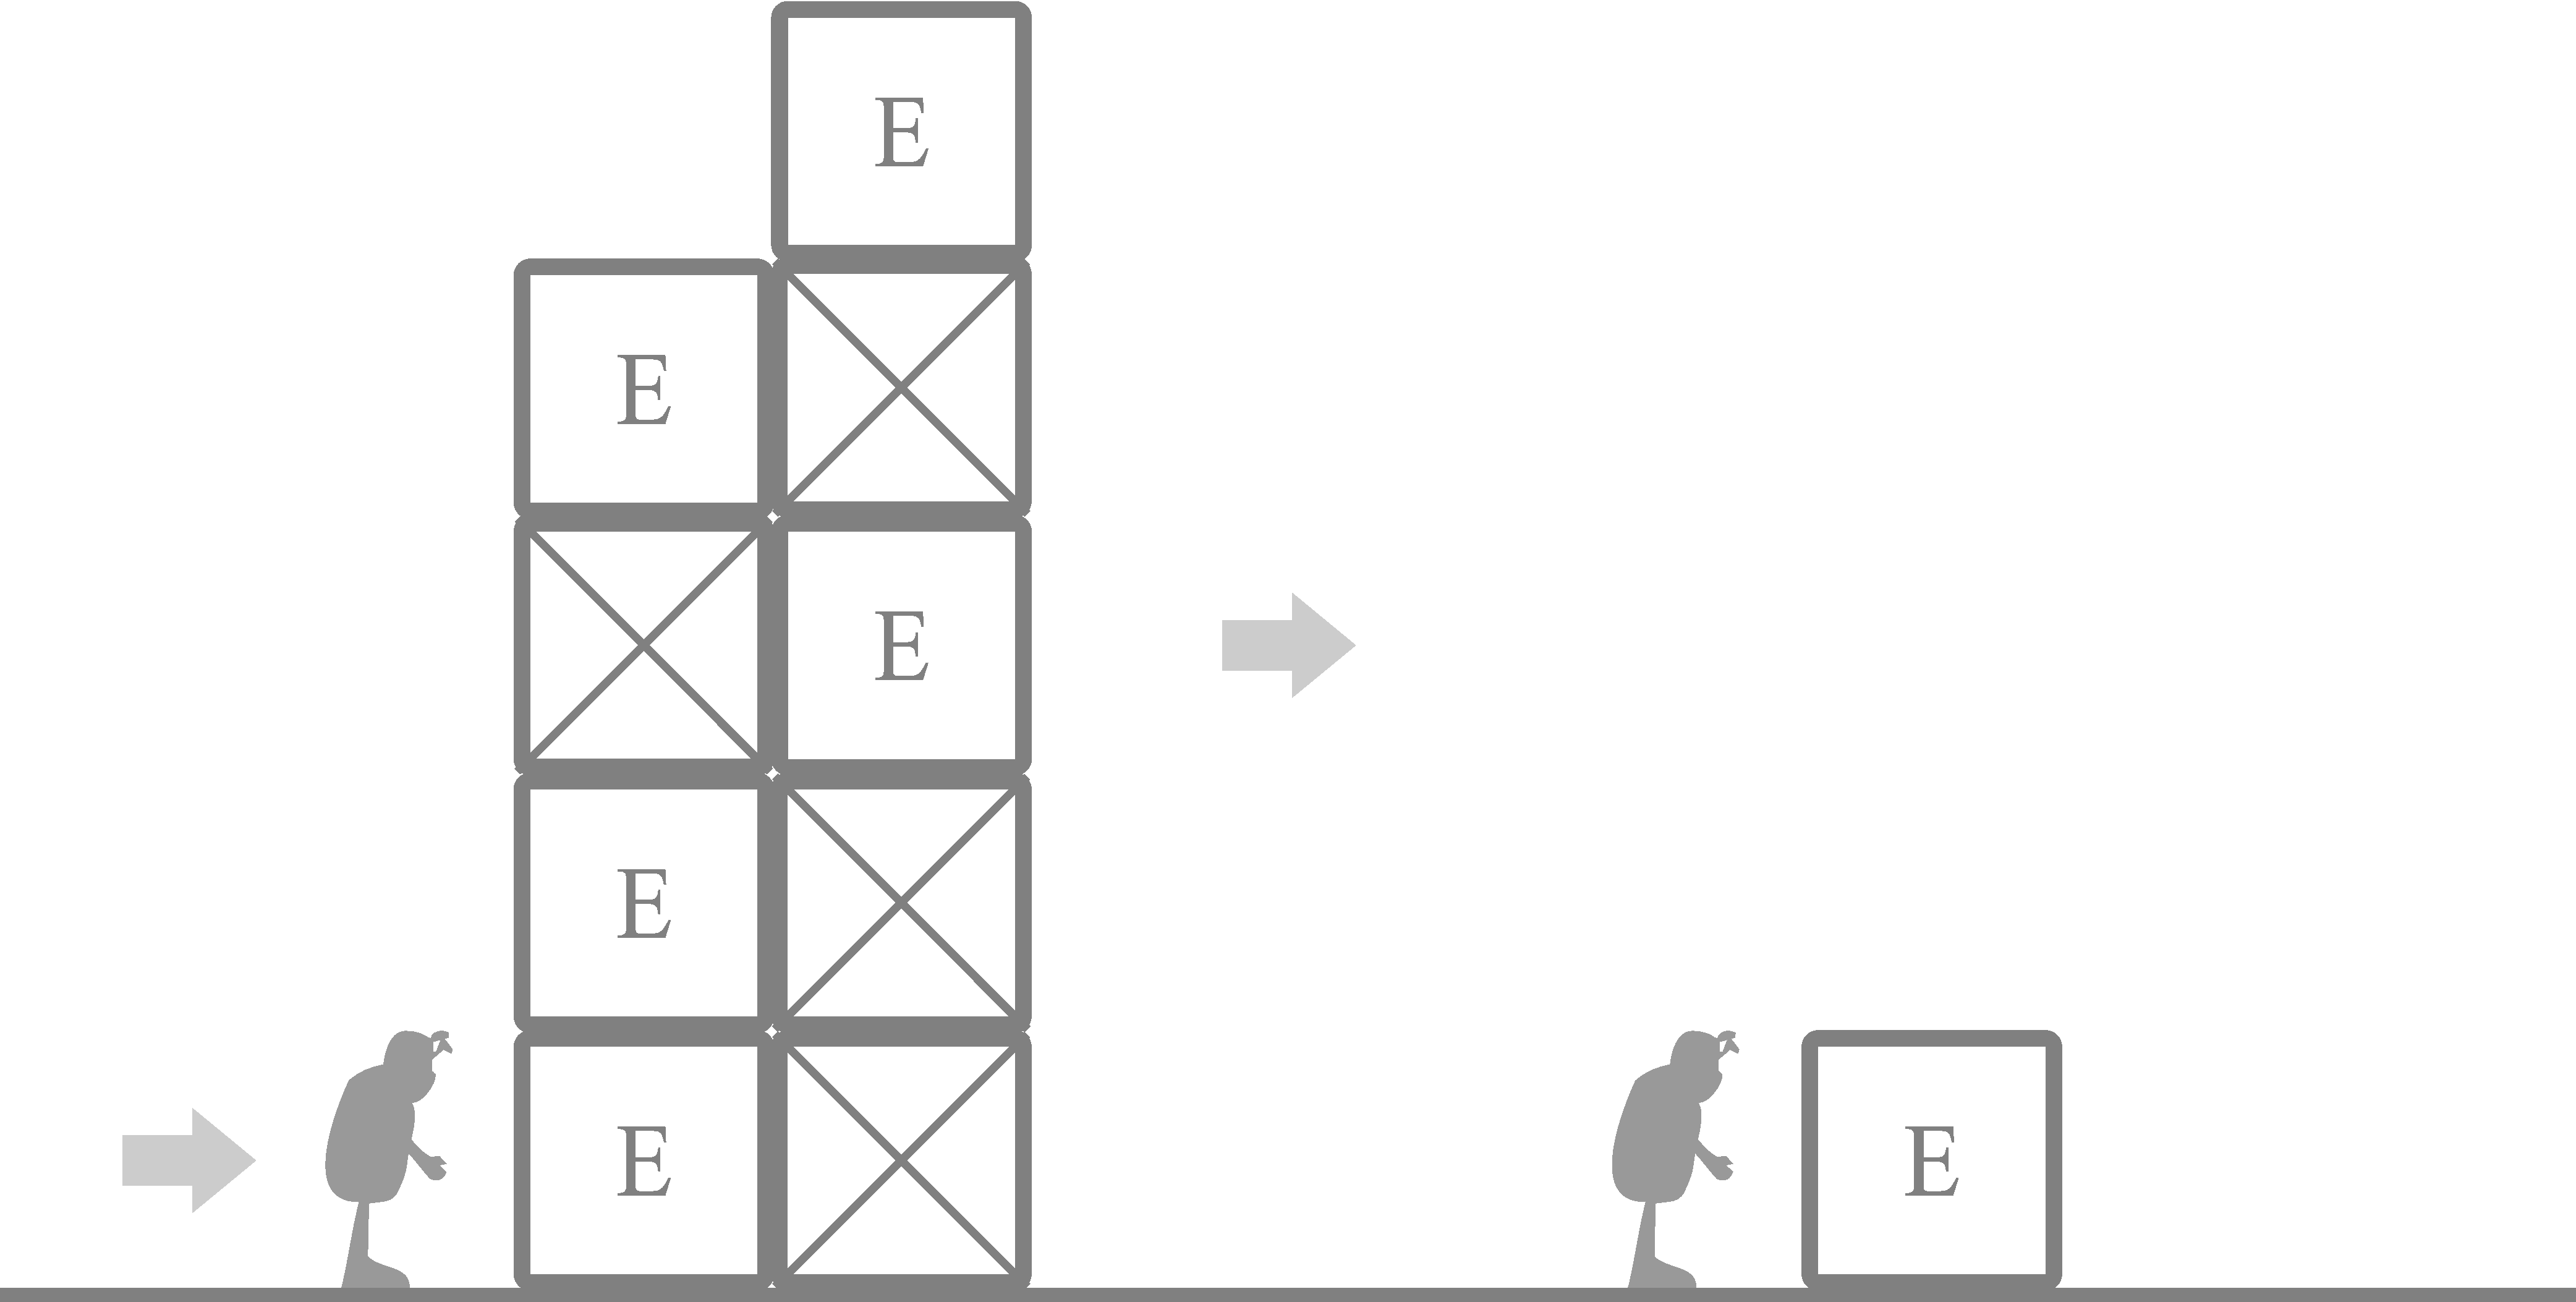
\includegraphics[width=0.8\textwidth]{bangDiagram}
\caption{Ukázka komplexního výbuchu}
\label{fig:bangDiagram}
\end{figure}

\section{Ovládání}
Berušky jsou vybírány pomocí kláves \keystroke{1} až \keystroke{5} a je s nimi pohybováno pomocí šipek. Důležité je ovládání kamery, která rotuje kolem momentálně vybrané berušky pohybem myši na okraj herní obrazovky. Pokud nemá uživatel přímou viditelnost na vybranou berušku, pak může objekty, které se mezi ním a beruškou nacházejí, nechat zprůhlednit pomocí mezerníku. Tlačítkem \Enter je pak pozice kamery přesunuta nad herní pole. 

\section{Vykreslování}
\label{section:navrhVykreslovani}
Informace týkající se technologie vykreslování jsou uvedeny v následujícím odstavci. Jejich přítomnost nechť čtenář bere pouze jako zajímavost, jelikož implementace hry, která je součástí této práce, probíhala nezávisle na hře původní. Jediným převzatým materiálem byla, jak se čtenář dále dozví, data pro zobrazení herní úrovně. 

V původní hře je celá scéna organizována jako strom hierarchických OBB obálek. Při vykreslování je pak strom procházen a je zjišťována viditelnost jednotlivých obálek. Osvětlovací model je kombinovaný z per-vertex shadingu a lightmap. Hra obsahuje také mnohé animace, které jsou u berušek realizovány jako objektové a pro zbytek objektů scény jako mesh animace. Aktuálně vyvíjená open-source varianta hry obsahuje také například zrcadlový rendering, kreslení odlesků, halo efekty, anisotropické filtrování textur, bump-mapping, komprimované textury a mip-mapping. Informace o uvedených technologiích vykreslování zde nebudou z důvodu omezeného rozsahu této práce uvedeny.

\section{Návrh webu}
Implementace této části nebyla přímou součástí této práce, a proto jejímu návrhu nebude věnován velký prostor. Návrh webu je možné vidět na diagramu~\ref{fig:web}. Web je rozdělen na 3~části a jejich popis se nachází v následujících odstavcích.


\subsection*{Menu}
Pomocí menu se volí kontexty obrazovky (viz. dále).
\subsection*{Obrazovka} Obrazovka je primárně určena k zobrazení aktuálně načtené herní úrovně. Pro ucelenost webu je však obrazovka využita i k zobrazení dalších informací a lze tedy rozpoznávat její jednotlivé kontexty. Těmi jsou:
	\begin{itemize}
	\item Hra

\item Informace o hře
\item Návod na hraní hry
\item Popis ovládání hry
	\end{itemize}
Při volbě herního kontextu se v rámci obrazovky zobrazí samotný element \texttt{<canvas>}, do kterého je vykreslována zvolená herní úroveň. V levém dolním rohu je zobrazen inventář aktuálně vybrané berušky a v rohu pravém je možné ovládat přehrávání herní hudby. Reakce na události vytvářené hráčem jsou zpracovány a o některých z nich je zobrazena notifikace, která tak dává hráči zpětnou vazbu. 
\subsection*{Výběr herních úrovní}
Tato část umožňuje uživateli vybrat z dostupných herních úrovní, které jsou následně vykreslovány do herního kontextu obrazovky. Mezi jednotlivými bloky pro výběr úrovně lze přecházet poklikem na šipky. Při jednom pokliku jsou úrovně posunuty o jeden blok a při pokliku dvojitém pak o bloky 4. Výběr by neměl obtěžovat hráče v okamžiku, kdy není potřeba. Proto je možné ho otevřít/skrýt pomocí tlačítka, které je umístěno ve spodní části obrazovky.


